\documentclass[../report.tex]{subfiles}

\begin{document}

\subsection{Implementation}

We provide a full implementation of the algorithms discussed prevously in Python and Cython\footnote{Code: \url{https://github.com/ManifoldFR/mva-optimaltransport/tree/master/project}}. Cython is used for performance-critical areas and provides a significant speedup.

\paragraph{Performance metrics.} To assess convergence, we use the multi-marginal Hilbert metric defined in \textcite[p.~16]{benamou2017generalizedIncompressible}
\begin{equation}
	d_{N,\calH}\left((a_k^{(n)}), (a_k^{(n+1)})\right) =
	\sum_{k=0}^{N} d_\calH\left(a_k^{(n)}, a_k^{(n+1)}\right)
\end{equation}
where $d_\calH(u,v) = \| \log(u) - \log(v) \|_V$ is the standard Hilbert metric (see \cite{peyr2018computational}). We also use it as an early stopping criterion for the Sinkhorn iterations.

We also compute after convergence of the Hilbert metric the relative $L^\infty$ error $L_n = \| \pi^0_\#\gamma^{(n)} - \rho_0\|_\infty/\| \rho_0 \|_\infty$ for the constraint $\pi^0_\# \gamma = \rho_0$.


\subsection{Crowd motion example}

We start by considering simple examples for crowd motion on a flat 2D grid, going from cases where a closed-form solution can be written to more complex cases where Sinkhorn iterations and computing multi-marginal convolutions become a concern. We look at how the penalty functions and constraints (obstacles, hard congestion, potential-based penalties) discussed in \textcite{benamou:hal-01295299} work out.

Our crowd motion model and formulation is the one suggested in \textcite{benamou:hal-01295299} (and earlier in \textcite{peyr2015entropic}) for modeling the problem. The cost structure is as follows: the terminal penalty is given by the constraints for the obstacles and congestion, and a potential $\Psi(x) = sd(x, \mathscr A)^{\beta}, s,\beta > 0$, related to the distance to a target set $\mathscr{A}$:
\begin{equation}
	G(\mu) = \langle \Psi, \mu\rangle + \imath_{0}(\mathds{1}_{\mathscr O}\mu)
	+ \imath_{[0,\bar{m}]}(\mu).
\end{equation}
\Cref{fig:CrowdExamplePotential} shows an example potential where we use the Euclidean distance to the target set $\mathscr{A}$.
In practice, we write $\bar{m}$ as a fraction of the initial maximum density $\|\rho_0\|_\infty$:
\[
	\bar{m} = \kappa \|\rho_0\|_\infty.
\]

The following proposition provides the $\KL$-proximal operators for a set of constraints and potentials that we will use. A proof is shown in \textcite{peyr2015entropic}.
\begin{prop}\label{prop:CrowdKLProx}~
\begin{itemize}
	\item The hard congestion constraint is $f(\mu) = \imath_{[0,\bar{m}]}(\mu)$. Its KL-projection is
	\begin{equation}
	\proj^{\KL}_f(\beta) = \min(\beta,\bar{m})
	\end{equation}
	where the minimum is taken element-wise.
	\item The KL-projection on the obstacle constraint $f(\mu) = \imath_{0} (\mathds{1}_\mathscr{O}\mu)$ is
	\begin{equation}
	\proj^{\KL}_f (\beta) = \beta \mathds{1}_{\Omega\backslash\mathscr{O}}
	\end{equation}
	\item Under a system of constraints with hard congestion and obstacles, a linear penalty function $f(\mu) = \langle\Psi, \mu\rangle + \imath_0(\mathds{1}_\mathscr{O}) + \imath_{[0,\bar{m}]}(\mu)$ has proximal operator
	\begin{equation}
	\prox^{\KL}_{f}(\beta) =
	\min(\beta\odot e^{-\Psi}, \bar{m}) \mathds{1}_{\Omega\backslash\mathscr{O}}
	\end{equation}
\end{itemize}
\end{prop}


\subsubsection{Two-marginal case}

We start with a very simplified approximation of the crowd displacement problem on $\Omega = [0, 1]^2$, with only two steps: the given initial distribution and the final distribution decided by the terminal penalty function $G$. 
Thus, the agents engage in a one-round mean-field game where they are only concerned with moving to regions with lower potential $\Psi$ -- as close as possible to $\mathscr{A}$ -- whilst obeying physical constraints related to the obstacles.

The discretized MFG problem with viscosity parameter $\epsilon = \sigma^2$ can be written as the following transport problem:
\begin{equation}\label{eq:2MargFuzzyObstacleObj}
\begin{aligned}
	&\inf_\gamma{} \langle \Psi, \gamma^T\mathds{1}\rangle + \KL(\gamma | \bfR) \\
	\suchthat\ & \gamma\mathds{1} = \rho_0, \quad \gamma^T\mathds{1} = \rho_1  \\
	& \rho_1 \leq \bar{m}, \quad \rho_1\odot \mathds{1}_{\mathscr{O}} = 0
	\end{aligned}
\end{equation}

\begin{prop}\label{thm:2MargFuzzyTarget}
Problem \eqref{eq:2MargFuzzyObstacleObj} can be solved in closed form: the Lagrange multiplier $u_0^*$ for the marginal law constraint satisfies
\begin{align*}
	a_0^* &= e^{u_0^*}  = \frac{\rho_0}{\bfR a^*_1}  \\
	a_1^* &= \min\left(\frac{\bar{m}}{\bfR a_0^*}, e^{-\Psi}\right)
\end{align*}
and the optimal coupling is $\gamma^* = \bfR\odot (a_0^* \otimes a_1^*)$.
It satisfies, as expected, that $\gamma^*_{i,j} = 0$ for all $j\in\mathscr{O}$. The final distribution of agents is
\[
	\rho_1 = \gamma^T\mathds{1} = a_1^* \odot \bfR a_0^*
\]
\end{prop}

 
\paragraph{Numerical experiment} We ran a numerical experiment by implementing the solutions given by \cref{thm:2MargFuzzyTarget} to the two-step MFG \eqref{eq:2MargFuzzyObstacleObj}. \Cref{fig:2MargFuzzyTransportObstacles} provides a representation of both. We also checked the results when removing the constraints: this leads to $a^*_1$ being obtainable in closed form with no iterations. We also looked at lowering the viscosity parameter $\sigma = \sqrt{\epsilon}$ (see \cref{fig:2MargFuzzyTransportRelaxedObst,fig:2MargFuzzyTransportLowVisc}). The results shown are satisfactory for the given potential $\Psi$: as expected the agents try to stay near the low-potential regions. But the results do not exactly look intuitive if we think of the problem as an exit problem: we see the need for appropriate potentials when modeling.

\begin{figure}[h]
	\centering
	\includegraphics[width=0.5\linewidth]{../project/images/naive_potential.png}
	\caption{Game domain $\Omega$ with set of obstacles $\mathscr{O}$ (dark grey), and contour of the potential function $\Psi$.} \label{fig:CrowdExamplePotential}	
\end{figure}


\begin{figure}[h]
	\centering
	\begin{subfigure}[t]{.70\linewidth}
	\includegraphics[width=\linewidth]{../project/images/fuzzy_transport_withobstacle.png}
	\caption{Result of the transport problem with enforcement of the obstacle constraints and viscosity parameter $\sigma=1$.}\label{fig:2MargFuzzyTransportObstacles}
	\end{subfigure}
	\begin{subfigure}[t]{.34\linewidth}
	\centering
	\includegraphics[width=\linewidth]{../project/images/fuzzy_transport_noobstacle.png}
	\caption{Final distribution $\rho^*_1$ without enforcing the obstacles. The mass of the distribution ``bleeds" through the obstacles. }\label{fig:2MargFuzzyTransportRelaxedObst}
	\end{subfigure}~
	\begin{subfigure}[t]{.34\linewidth}
	\centering
	\includegraphics[width=\linewidth]{../project/images/fuzzy_transport_lowvisc.png}
	\caption{Obstacles are constrained as in \cref{fig:2MargFuzzyTransportObstacles}, but with lower viscosity.}\label{fig:2MargFuzzyTransportLowVisc}
	\end{subfigure}
	\caption{Numerical solution of the two-step MFG problem \eqref{eq:2MargFuzzyObstacleObj}, with a few variations.}\label{fig:2MargFuzzyTransportMarginals}
\end{figure}

\begin{remark}[A more realistic potential]\label{rem:SmartPotential}
In a room evacuation scenario, for instance, agents would seek to minimize the time-to-exit: the literature shows this leads to the Eikonal equation $|\nabla u(x)| = 1/f(x)$, a kind of Hamilton-Jacobi PDE. We computed the adequate potential shown \cref{fig:CrowdShortedPathPotential} using the Fast Sweeping method \parencite{Zhao2004AFS}. The solution to the associated discrete 2-step MFG is shown \cref{fig:2MargEikonalGame}.

Of course, another way of modeling the exit problem we're considering would be to change the objective \eqref{eq:ControlObjective} to minimizing the stopping time corresponding to the exit, and deduce new MFG equations: this is explored by \textcite{benamou:hal-01295299} who derive a variational formulation for that problem.
\end{remark}

\begin{figure}[h]
	\centering
	\begin{subfigure}[b]{.4\linewidth}
		\centering
		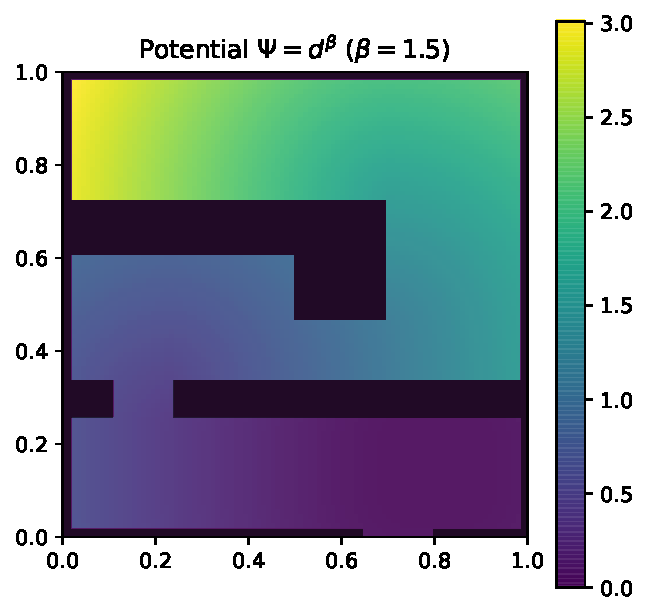
\includegraphics[width=\linewidth]{../project/images/multimarg_room1/room_potential.pdf}
		\caption{Domain and potential associated with the fastest path distance.}\label{fig:CrowdShortedPathPotential}
	\end{subfigure}~
	\begin{subfigure}[b]{.36\linewidth}
		\centering
		\includegraphics[width=\linewidth]{../project/images/eikonal_transport_lowvisc.png}
		\caption{Optimal terminal distribution $\rho^*_1$ of the discrete MFG with the potential from \cref{fig:CrowdShortedPathPotential}.}\label{fig:2MargEikonalGame}
	\end{subfigure}
	\caption{Setup and solution for the discrete MFG using the time-to-exit potential discussed in \cref{rem:SmartPotential}.}
\end{figure}


\subsubsection{Three time steps}

We now go up to three marginals $(\rho_0,\rho_1,\rho_2)$. We assign to the single intermediate marginal $\rho_1$ the same constraints: congestion $\rho_1 \leq \bar{m}$ and the obstacles. The primal problem then reads
\begin{equation}
\begin{aligned}
	&\inf_{\gamma,\rho_1,\rho_2}{} \langle \Psi, \rho_2\rangle + \KL(\gamma | \bfR) \\
	\suchthat \ & \pi^k_\#\gamma = \rho_k,\; k = 0,1,2 \\
	& \rho_1 \leq \bar{m}, \quad \rho_1\odot\mathds{1}_{\mathscr O} = 0\\
	& \rho_2 \leq \bar{m}, \quad \rho_2\odot\mathds{1}_{\mathscr O} = 0
\end{aligned}
\end{equation}

\begin{prop}
The Lagrange multipliers $u_i^*$ at the optimum satisfy the fixed-point conditions:
\begin{align*}
	&a_0^* = \frac{\rho_0}{\bfR[\,\cdot\,, a_1^*, a_2^*]} \\
	&a_1^* = \min\left(
	\frac{\bar{m}}{\bfR[a_0^*, \,\cdot\,, a_2^*]}, 1\right) \\
	&a_2^* = \min\left(
	\frac{\bar{m}}{\bfR[a_0^*, a_1^*, \,\cdot\,]}, e^{-\Psi}
	\right)
\end{align*}
where $a_i^* = \exp(u_i^*)$ are supported on $\Omega\backslash\mathscr{O}$ and we denote $\bfR[\cdot,\cdot,\cdot]$ tensor contraction by $\bfR$.
The marginals are given by
\[
\begin{aligned}
	\rho_1^* &=
	a_1^* \odot
	\bfR[a_0^*, \,\cdot\,, a_2^*] =
	a_1^* \odot
	(\mathbf{P}^Ta_0^*) \odot
	(\mathbf{P}a_2^*) \\
	\rho_2^* &= 
	a_2^* \odot \bfR[a_0^*, a_1^*, \,\cdot\,]
	= a_2^* \odot
	\mathbf{P}^T
	(a_1^* \odot \mathbf{P}^Ta_0^*)
\end{aligned}
\]
\end{prop}



The fixed point can be solved using an iterative scheme just like in the generalized Sinkhorn algorithm from \cref{algo:Sinkhorn}.
The same bottlenecks in computing the sum-product contractions appear, and have already been expanded upon in \cref{sec:PartialDiscret}.

\paragraph{Numerical experiment.} An example on the domain $\Omega$ from before is given \cref{fig:3MargTransport}. Qualitatively, the result is not entirely satisfying: it looks like some of the mass ``bleeds" through the boundary. This might be the case due to the time step being too coarse.

\begin{figure}[h]
	\centering
	\includegraphics[width=.8\linewidth]{../project/images/three_marginal_room1.png}
	\caption{Three time step discrete MFG.}\label{fig:3MargTransport}
\end{figure}


\subsubsection{Full $N$-marginal case}

Implementation of the full multimarginal problem is straightforward once given an efficient implementation of \cref{algo:EfficientIntegral}, which is the core effort when computing the Sinkhorn iterations from the algorithm in \cref{algo:Sinkhorn}.


\paragraph{Initial example.} The setup is the same as in the prequel. The result is given \cref{fig:NMargEx1Soltn}. The grid size was $M = 101^2$, $30$ time steps, viscosity $\sigma = 0.04$. Convergence of the Hilbert metric was obtained in $12.8$ seconds on a 2.6GHz Intel Core i7 processor. For this number of iterations, the relative $L^\infty$ error for the $\rho_0$ constraint is of order $10^{-10}$.

\begin{figure}[h]
	\centering
	\begin{subfigure}[c]{.4\linewidth}
	\includegraphics[width=\linewidth]{../project/images/multimarg_room1/congestion_plot.pdf}
	\caption{Congestion plot of $(\|\rho_t\|_\infty)_t$.}
	\end{subfigure}~
	\begin{subfigure}[c]{.4\linewidth}
		\includegraphics[width=\linewidth]{../project/images/multimarg_room1/hilbert_convergence.png}
		\caption{Convergence of the Hilbert metric.}
	\end{subfigure}
	\begin{subfigure}[c]{.8\linewidth}
		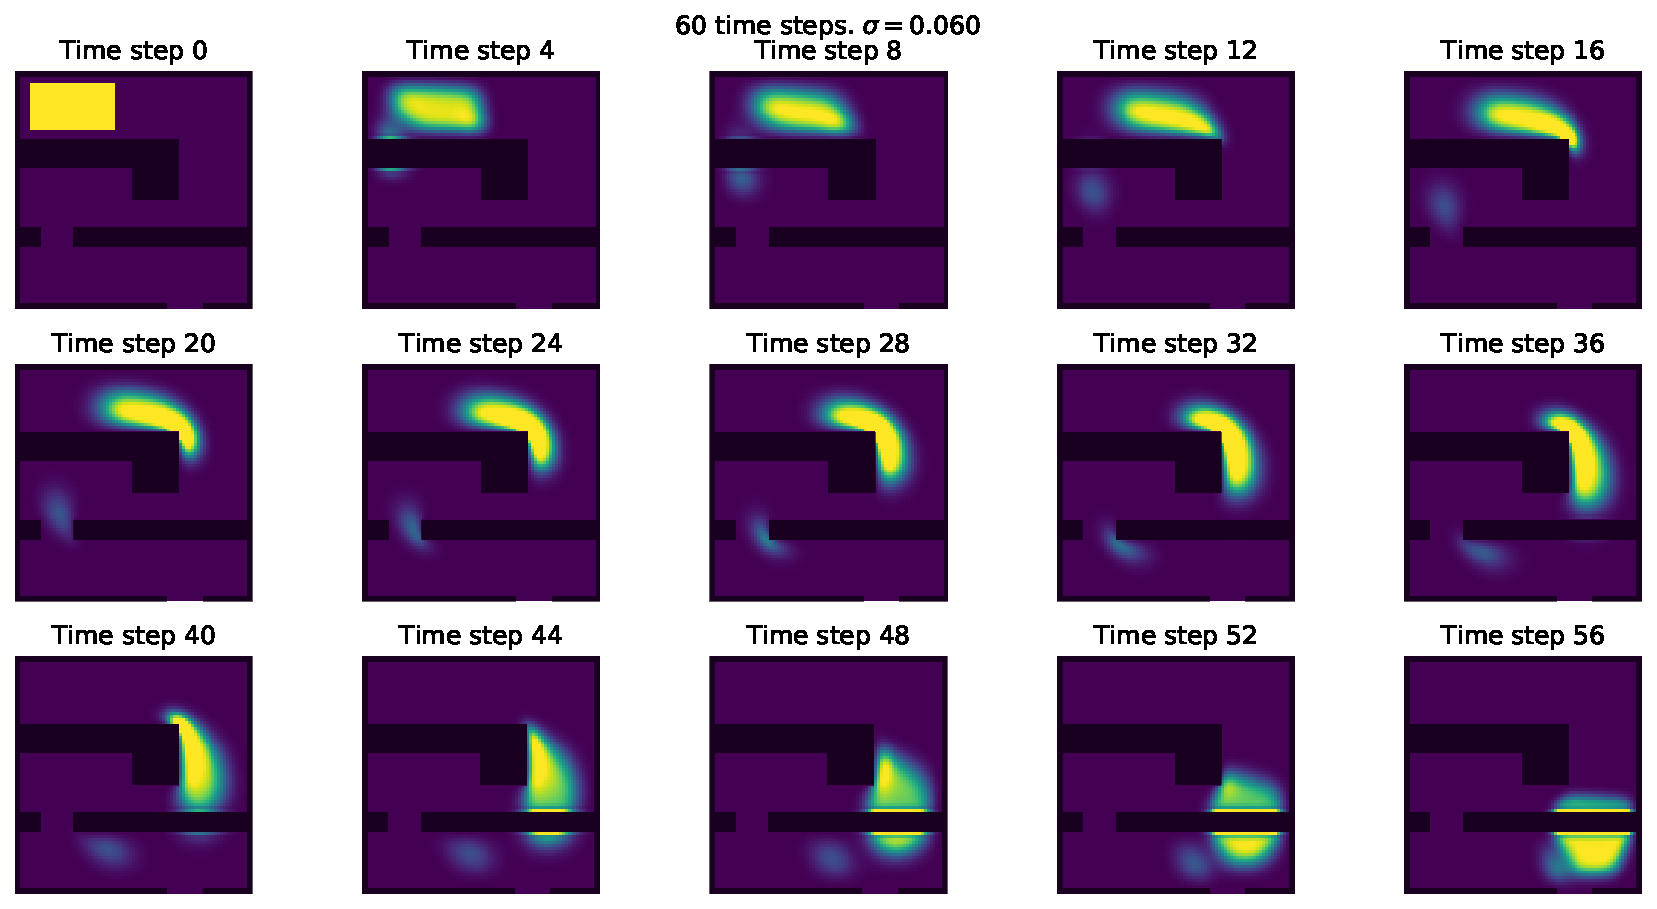
\includegraphics[width=\linewidth]{../project/images/multimarg_room1/multimarg_transport.pdf}
		\caption{Numerical solution of the MFG for the first room.}\label{fig:NMargEx1Soltn}
	\end{subfigure}
	\caption{Numerical results for the full crowd model. First room.}
\end{figure}

\begin{comment}
\begin{figure}[h]
	\centering
	\begin{subfigure}[c]{.4\linewidth}
		\includegraphics[width=\linewidth]{../project/images/multimarg_room2/congestion_plot.pdf}
		\caption{Congestion plot for the second room.}\label{fig:Room2CongestPlot}
	\end{subfigure}~
	\begin{subfigure}[c]{.4\linewidth}
		\includegraphics[width=\linewidth]{../project/images/multimarg_room2/hilbert_convergence.png}
		\caption{Convergence of the Hilbert metric.}
	\end{subfigure}
	\begin{subfigure}[c]{.6\linewidth}
		\includegraphics[width=\linewidth]{../project/images/multimarg_room2/multimarg_transport.pdf}
		\caption{Numerical solution of the MFG for the second example.}\label{fig:NMargEx2}
	\end{subfigure}
\end{figure}
\end{comment}

\begin{comment}
\paragraph{Second room.} The setup is given in \cref{fig:NMarg2DomainPot}: the new domain is $\Omega = [0,1] \times [0,2]$ and consists of two rooms separated by a long but narrow hallway with a singular choke point. We use a viscosity parameter $\sigma = 0.1$. Results are given \cref{fig:NMargEx2}. The constraints and costs are identical as before. The grid size was $M = 51 \times 101$, and the result was obtained with $150$ Sinkhorn iterations, which took about $118$ seconds on a 2.6GHz Intel Core i7 processor. The final relative $L^\infty$ error on the $\rho_0$ constraint was of order $10^{-4}$. However, the congestion plot \cref{fig:Room2CongestPlot} suggests that the algorithm hasn't exactly converged.
\end{comment}

\begin{comment}
\begin{figure}[h]
	\centering
	\begin{subfigure}[b]{.3\linewidth}
		\includegraphics[width=\linewidth]{../project/images/multimarg_room2/room_setup.pdf}
	\end{subfigure}~
	\begin{subfigure}[b]{.39\linewidth}
		\includegraphics[width=\linewidth]{../project/images/multimarg_room2/room_potential.pdf}
	\end{subfigure}
	\caption{Domain, initial and target agent distributions, and associated potential $\Psi$ for the multi-marginal problem. The initial distribution $\rho_0$ is in blue, the objective is in red.}\label{fig:NMarg2DomainPot}
\end{figure}
\end{comment}



\paragraph{Second room.} The setup is given \cref{fig:Room3}. Computation on a $M=101^2$ grid with $N=30$ time steps and viscosity $\sigma = 0.04$ took $16$ seconds for convergence. The $L^\infty$ constraint relative error was of order $10^{-10}$.

We observe the ``bleeding" problem: some of the mass decides to clip through obstacles and walk through walls. This is obviously not a physically acceptable solution. It seems like the new domain is much more difficult to handle. Using a more appropriate kernel $\bfR$ might be necessary.

\begin{figure}[h]
	\centering
	\begin{subfigure}[c]{.4\linewidth}
		\includegraphics[width=\linewidth]{../project/images/multimarg_room3/room_setup.pdf}	
	\end{subfigure}~
	\begin{subfigure}[c]{.45\linewidth}
		\includegraphics[width=\linewidth]{../project/images/multimarg_room3/room_potential.pdf}	
	\end{subfigure}
	\caption{Domain, setup and potential for the second room.}\label{fig:Room3}
\end{figure}

\begin{figure}[h]
	\centering
	\begin{subfigure}[c]{.4\linewidth}
		\includegraphics[width=\linewidth]{../project/images/multimarg_room3/congestion_plot.pdf}\caption{Congestion plot for the second room.}
	\end{subfigure}~
	\begin{subfigure}[c]{.4\linewidth}
		\includegraphics[width=\linewidth]{../project/images/multimarg_room3/hilbert_convergence.png}
		\caption{Convergence of the Hilbert metric.}
	\end{subfigure}
	\begin{subfigure}[c]{.8\linewidth}
		\includegraphics[width=\linewidth]{../project/images/multimarg_room3/multimarg_transport.pdf}
		\caption{Numerical solution of the MFG in the second example room.}\label{fig:NMargEx3}
	\end{subfigure}
	\caption{Numerical results for the second room.}\label{fig:Room3Results}
\end{figure}


\end{document}
